%================
\chapter{The Limit of ATM}
%================

\section{Introduction}

これまで、様々な形で我らがATM\index{ATM@ATM}の特性について述べてきた。特に、異なるATM同士の接近により、無限の深さの井戸型ポテンシャルを持って負の方向にばらぼんばらぼんばらぼんぬ\index{ばらぼんぬ@ばらぼんぬ}
である(第2章参照)。
\par
しかし、近年四菱USA(四菱大阪ユニバーサル・スタディウォ・アバン)\index{よつびしゆーえすえー@四菱USA(四菱大阪ユニバーサル・スタディウォ・アバン)}によって行われた最新の研究により、いい加減ATM\index{ATM@ATM}にも限界が存在する事が判明した。本章ではその詳細について述べていく。
\par
事の発端は、ATM\index{ATM@ATM}の自動送信投下である(図\ref{taihennya})。2018年9月4日、LINEグループ「オガワ」にてATMからダイレクトメッセージが投下された。またこの本文と同時に、図\ref{taihennya2}のようなものが添付された。
毎度毎度ATMが滑り散らかして対応に困っていた我々は、四菱USAと協力のもと、ATMの限界を調査していく事にした。
その方法は、主にこちらから質問などを通して会話をいくつかする事で、その反応を見るというものである。
それらの質問はある種の"パス"であり、返答次第ではATMは革命的な面白発言により我々を会話の"ゴール"に導くのか、はたまた奈落の闇へと落とし込むのか、無限の可能性が秘めているという事が期待されるのである。
知らんけど。\\
 
\begin{figure}[H]
\centering
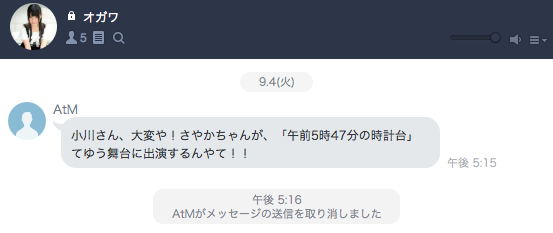
\includegraphics[clip,scale=0.5]{taihennya.png}
\caption{LINEグループ「オガワ」にて、ATMから定期的に送られてくるDMのような投稿。学生の頃から無視ってたがまさか卒業してからも送られてくるとは。そして何のメッセージを取り消したのか。果たして仕事をしているのか。}
\label{taihennya}
\end{figure}

\begin{figure}[H]
\centering
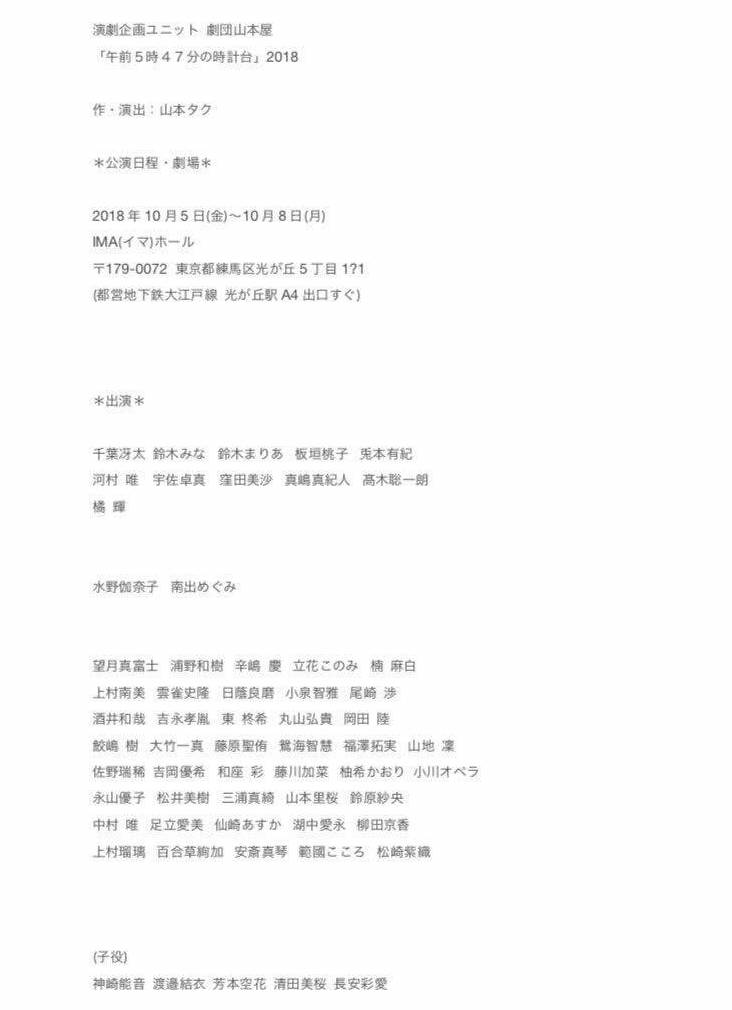
\includegraphics[clip,scale=0.5]{taihennya2.jpg}
\caption{まあどうでもいいし、これを送信するためにいちいちスクショしたりしてると考えると、果たして仕事をしているのか。}
\label{taihennya2}
\end{figure}

まずはじめに、「ちょっとその日は忙しいです$\sf{ (´\_ゝ`)}$」と軽いジャブを打ってみた。また、それと並行して図\ref{taihennya3}に示す画像を添付した。


\begin{figure}[H]
\centering
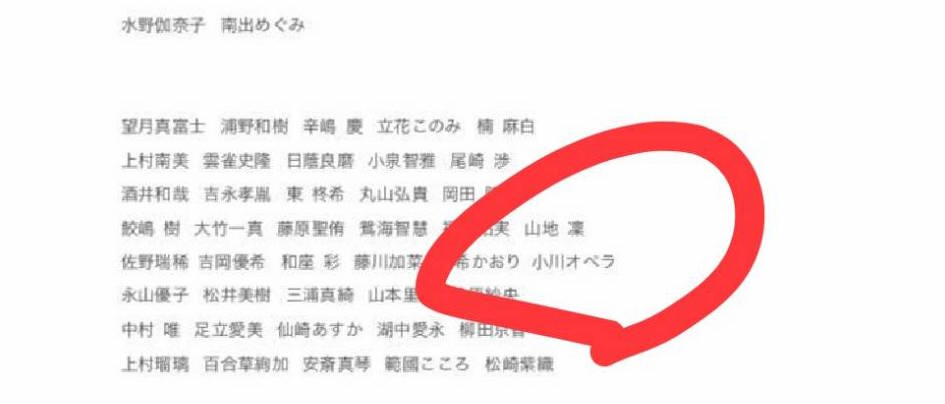
\includegraphics[clip,scale=0.35]{taihennya3.jpg}
\caption{なんかよく見たら「小川」がいたので、あえてこのマークだけして何かコメントをいただくべく"パス"を出した。果たしてATM限界はあるのか、または、あるのか。}
\label{taihennya3}
\end{figure}

すると、ATMは以下のように返事をした(図\ref{taihennya4})。安定のウザさである。まず絵文字を使っているのも腹たつし、一体どの立場でこの発言をしているのか。\\
 

\begin{figure}[H]
\centering
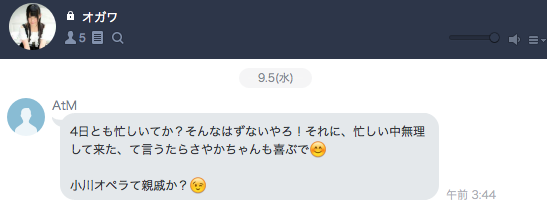
\includegraphics[clip,scale=0.5]{taihennya4.png}
\caption{ヒント:返信時間}
\label{taihennya4}
\end{figure}

ここで我々は、いい加減どうやっても面白くならないのではと感じ、偉大なる重症患者\index{じゅうしょうかんじゃ@重症患者}クイズタケオネア氏(100万歳)\index{くいずたけおねあし@クイズタケオネア氏(100万歳)}
に助けを求めた(図\ref{taihennya6})。ここで得られた質問をすることで、決定的なATMの限界を追求する事ができると確信したのである。

\begin{figure}[H]
\centering
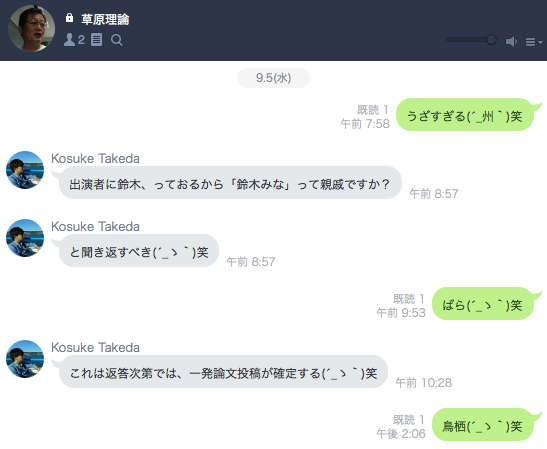
\includegraphics[clip,scale=0.5]{taihennya6.png}
\caption{やはりクイズタケオネア氏は偉大である。CERNにいる事を考慮すると若干、返信時間がおかしい気もするが。}
\label{taihennya6}
\end{figure}

以上を参考にし、「鈴木みなって親戚ですか?$\sf{ (´\_ゝ`)}$」という質問とともに図\ref{taihennya5}を添付した。
\begin{figure}[H]
\centering
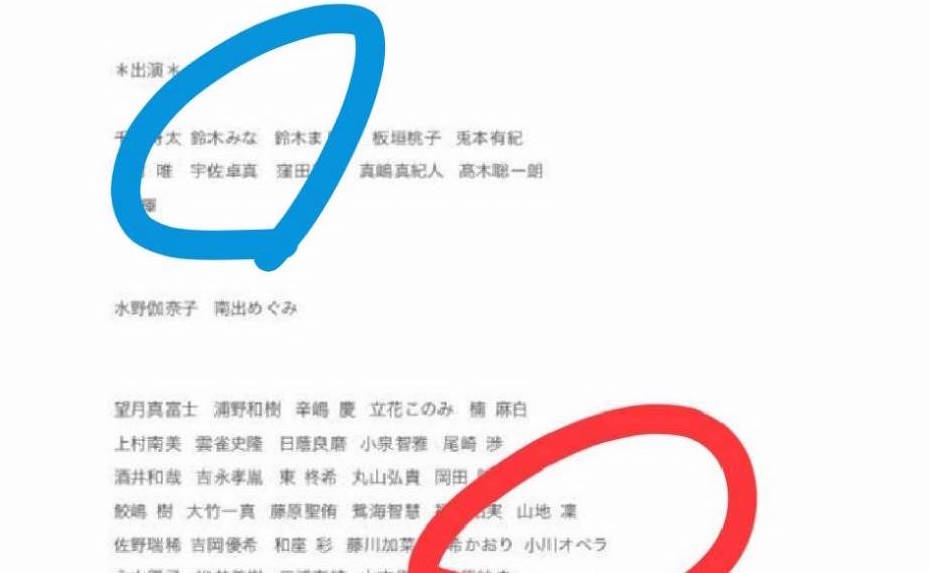
\includegraphics[clip,scale=0.35]{taihennya5.jpg}
\caption{よくみたらこの小川の左にかおりいるやんけ}
\label{taihennya5}
\end{figure}

以上の結果、以下のような返信が来たのである。
\begin{figure}[H]
\centering
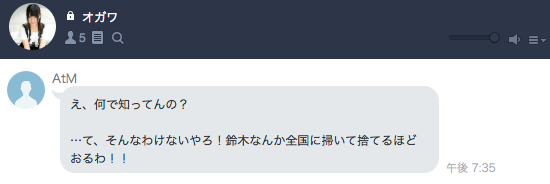
\includegraphics[clip,scale=0.6]{taihennya7.png}
\caption{ATMの限界を初観測した瞬間である。}
\label{taihennya7}
\end{figure}

これはひどい。これこそがまさにATMの限界を迎えた瞬間である。まずはこのクソ寒いノリツッコミである。ありきたりな質問に対しありきたりな返事をした時点でもはやこの文章を読む価値はないのだが、気持ちノッた後に改行2回だけしただけで突っ込んでしまうセンスのなさとしょうもないツッコミである。関西というお笑い文化が根付いている地域に住み、なおかつおしゃべりが活発な若者と日々関わる機会のある恵まれた環境に身を投じているにもかかわらず、この有様である。如何にATMが、自分が置かれている環境に感謝せず、なおかつ現状に満足せずに日々の鍛錬を行うために「会話」という形で有効活用していないかが分かる。まがりなりにも国立大学の理学研究科の助教という役職に就いているにもかかわらず、しかも世界的な規模の分野である素粒子実験の業界に身を投じているにもかかわらず、普段からのコミュニケーションを怠っているがために起こった過ちであり、言語道断の誠に遺憾である。もはやこの掃いて捨てるほどいる鈴木とはATM自身の事ではないだろうか、自己紹介なのではないか、と思わざるを得ないのである。\\
またこの瞬間、我々は四菱USA(四菱大阪ユニバーサル・スタディウォ・アバン)\index{よつびしゆーえすえー@四菱USA(四菱大阪ユニバーサル・スタディウォ・アバン)}との共同実験を終了した。


\section{Summary}
まあまとめると以下の通りである。知らんけど。ばらっっっっっっっ\index{ばらっっっっっ@ばらっっっっっ}

\begin{itembox}[c]{$\sf{ (´\_ゝ`)}$}
ATMの預金残高は掃いて捨てるほどある。
\end{itembox}


